% Winter cycling on rue de Terrebonne and the days snow is loaded.
% Analysis of the counter data released under access request 2026-300,
% joined to Environment Canada weather and the City's snow-removal records.
% Compile with pdflatex (twice).
\documentclass[11pt,letterpaper]{article}
\usepackage[T1]{fontenc}
\usepackage[utf8]{inputenc}
\usepackage[scaled=0.95]{helvet}
\renewcommand{\familydefault}{\sfdefault}
\usepackage[letterpaper,top=0.9in,bottom=0.95in,left=1in,right=1in]{geometry}
\usepackage{microtype}
\usepackage{enumitem}
\usepackage{titlesec}
\usepackage{fancyhdr}
\usepackage{xcolor}
\usepackage{booktabs}
\usepackage{amsmath}
\usepackage{graphicx}
\usepackage{array}
\usepackage[hidelinks]{hyperref}
\urlstyle{same}
\newcommand{\docversion}{2026-10-21-19-46-05} % set by build (America/Toronto)
\hypersetup{pdfsubject={version \docversion}}

\setlength{\parindent}{0pt}
\setlength{\parskip}{0.5em}
\linespread{1.03}

\titleformat{\section}{\normalfont\large\bfseries}{\thesection}{0.6em}{}[\vspace{1pt}\titlerule]
\titlespacing*{\section}{0pt}{1.1em}{0.4em}
\titleformat{\subsection}{\normalfont\bfseries}{\thesubsection}{0.6em}{}
\titlespacing*{\subsection}{0pt}{0.8em}{0.25em}

\pagestyle{fancy}
\fancyhf{}
\renewcommand{\headrulewidth}{0pt}
\fancyfoot[C]{\footnotesize\color{gray}Access request 2026-300 -- winter cycling and snow-loading days -- page \thepage}
\fancyfoot[R]{\tiny\color{gray}v.\,\docversion}

\newcommand{\repourl}{https://github.com/OpenMobilityData/Terrebonne-access-requests}
\newcommand{\repo}[1]{\href{\repourl}{#1}}
\newcommand{\doc}[2]{\href{\repourl/blob/main/#1}{#2}}
\newcommand{\pagesurl}{https://openmobilitydata.github.io/Terrebonne-access-requests}
\expandafter\def\csname bundle01\endcsname{2026-581/raw/01_emails_mandate_counts.pdf}
\newcommand{\pgl}[3]{\href{\pagesurl/\csname bundle#1\endcsname\#page=#2}{\textsf{\small[#1, p.~#3]}}}
\newcommand{\pg}[2]{\pgl{#1}{#2}{#2}}

\begin{document}

\begin{center}
{\Large\bfseries Winter cycling on rue de Terrebonne and the days snow is loaded}\\[0.4em]
{\large What the borough's counter, Environment Canada and the City's snow-removal records show for winter 2025--26}\\[0.6em]
Richard Hoge, C\^ote-des-Neiges--Notre-Dame-de-Gr\^ace -- October 13, 2026\\
Published with the source data at \repo{\repourl}
\end{center}

\section*{Summary}

The borough of C\^ote-des-Neiges--Notre-Dame-de-Gr\^ace has announced that
one direction of the protected bike lane on rue de Terrebonne will be
converted to parking each winter. No dates appear in any borough document;
the councillor for Loyola has described the season as ``December to
March'' and the reopening as set by ``the data and the weather'' (CBC
\emph{Daybreak}, October~9, 2026). This note takes December~1 to March~31
as the winter. The engineering
mandate behind the announcement also listed a narrower option, closing the
lane ``en p\'eriode de d\'eneigement seulement'' \pg{01}{10}. This note
measures what each option would have meant for cyclists last winter, using
three public records: the borough's own continuous bicycle counter at
Terrebonne and Kensington, released under access request 2026-300; daily
weather from Environment Canada; and the City of Montr\'eal's open record of
every truckload of snow hauled from the borough. Nothing is modelled; every
figure is a count on a day that happened.

Two things stand out. Most winter days have no snow, those are the days
with the most cycling, and on those days a parking lane in place of the
bike lane serves no snow-related purpose while every eastbound trip is
ridden in a traffic lane between parked cars. And on the days that do have
snow, cycling continues at close to its usual winter level; on those days
the lane would be closed under either option, and the trips are made on
the roadway at its worst.

\begin{enumerate}[nosep]
  \item \begin{minipage}[t]{\linewidth}\textbf{Last winter 4{,}891 bicycle trips were counted at Kensington
    between December~1 and March~31, 2{,}783 of them eastbound.} Under an
    all-winter conversion every eastbound trip is a trip in mixed traffic.
    Under a closure limited to snow-loading days, the number is 410 on the
    borough's loading days (15\%) and 548 on the loading days of the
    contract sector that contains Terrebonne (20\%).\end{minipage}\vspace{0.35em}
  \item \begin{minipage}[t]{\linewidth}\textbf{Most winter cycling happens on days with no snow.} 1{,}699
    eastbound trips, 61\%, were on the 67 days with no snowfall at all;
    83\% on days with less than 2.5~cm.\end{minipage}\vspace{0.35em}
  \item \begin{minipage}[t]{\linewidth}\textbf{The result does not depend on the winter.} Winter 2025--26 was
    light: 7.3~million~m$^3$ of snow hauled city-wide, the second-lowest
    of the eleven seasons in the City's record. Applying each of those
    eleven seasons' loading calendars to last winter's daily counts gives
    a storm-day share of 9\% to 24\%, median 18\%.\end{minipage}\vspace{0.35em}
  \item \begin{minipage}[t]{\linewidth}\textbf{Within deep winter, loading days carry about the same
    cycling as other days.} From December to February eastbound trips
    averaged 17 a day on the borough's loading days and 18 on other days;
    the full-season difference (17 against 25) comes from March, when use
    rises and snow is scarce. Winter cyclists ride through loading
    operations; they do not stay home for them.\end{minipage}\vspace{0.35em}
  \item \begin{minipage}[t]{\linewidth}\textbf{The counter's westbound channel degraded around March~1,
    2026.} A camera on the same street confirms it. The figures above
    treat the eastbound counts as lower bounds from that date; on the firm
    window, December~1 to February~28, the storm-day shares are 23\% and
    28\% and the zero-snow share 48\%. The conclusions are the same on
    either window.\end{minipage}
\end{enumerate}

\section{Data}

\textbf{Bicycle counts.} The borough operates an Eco-Counter ZELT EVO
inductive-loop counter on Terrebonne at Kensington, in service since
July~26, 2025. Its hourly record by direction, July~26, 2025 to May~11,
2026, was released on June~4, 2026 under access request 2026-300
(\doc{2026-300/raw/}{raw/}); the equipment documentation was released under
request 2025-697. Summed to days, the record matches exactly the daily
totals the borough released on October~9, 2026 in file 2026-581
\pgl{01}{74}{74--81}: December~1 to March~31, 4{,}891 trips, 2{,}783
eastbound and 2{,}108 westbound. Over the counter's first full year,
July~26, 2025 to July~25, 2026, the same daily table gives 135{,}276
bicycle passages (371 a day) and 501{,}817 motor vehicles (1{,}375 a
day): one bicycle for every 3.7 motor vehicles, or 21\% of all vehicles
counted. The bicycle figure is a lower bound: May~29--31, 2026 are three
days of zero (an outage), and the westbound channel's detection degraded
from about March~1, 2026 (see Limits). Eastbound is taken here as the direction
that would lose its lane: on CBC \emph{Daybreak} on October~9 the
councillor for Loyola said the orientation given to the services was ``to
favour the side that will be against traffic to remain during winter''
[00:38], as he had said in answer to questions at the October~6 meeting
and earlier to the APC-NDG; the lane running with motor traffic at
Kensington is eastbound (west of Cavendish, where the one-way reverses, it
is westbound). If the westbound lane were converted instead,
every figure scales by 2{,}108/2{,}783 and no conclusion changes.

\textbf{Weather.} Environment and Climate Change Canada daily data for
Montr\'eal/Pierre Elliott Trudeau International Airport (climate ID
7025251): total snowfall, snow on the ground, temperature.\footnote{ECCC
historical climate data, \url{https://climate.weather.gc.ca}; the two
annual files are in \doc{2026-300/derived/}{derived/}.} One missing day
(March~8) is treated as no snow.

\textbf{Snow loading.} The City publishes every snow-removal truckload with
its loading time, contract sector, borough, dump site and volume
(\emph{Contrats et transactions de d\'eneigement}, CC-BY
4.0).\footnote{\url{https://donnees.montreal.ca/dataset/contrats-transaction-deneigement}}
Filtered to borough code CDN and summed by day, it gives the borough's
loading days for every season since 2015--16. The City's sector polygons
for 2025--26\footnote{\emph{Secteurs de d\'eneigement},
\url{https://donnees.montreal.ca/dataset/secteur-deneigement}.} place the
lane in contract sector CDN-301 from its west end, just west of Belmore,
to between Royal and Draper, about 1.8 of its 2.4~km, the counter
included; the last blocks, Draper to Girouard (about 0.55~km), are in
sector CDN-111, and the Girouard intersection lies on the boundary with
CDN-112 (intersections from the City's g\'eobase; the check is
\texttt{terrebonne\_sector.py}). A
day with 100 or more loads in the borough, or 40 or more in the sector, is
counted as a loading day; full operations run at several hundred loads a
day and the tails below those thresholds are mop-up. In 2025--26 this gives
24 borough loading days in six episodes (December~12--16 and 28--31,
January~8--9, 17--21 and 27--31, February~27 to March~2), matching the six
operations the City announced, and 30 days for sector CDN-301, whose
operations run a day or two longer.

\section{Method}

Let $n_d$ be the eastbound trips counted on day $d$ of the season $S$
(December~1 to March~31, 121 days). Under an all-winter conversion the
exposure is $E_{\text{all}} = \sum_{d\in S} n_d = 2{,}783$. Under a closure
limited to a set of storm days $\mathcal{D}$, it is $E_{\mathcal{D}} =
\sum_{d\in\mathcal{D}} n_d$. Since the City has not said how a storm
closure would be defined, $\mathcal{D}$ is computed under several
definitions, from a single snow day to every day with any loading activity
in the borough. To test the dependence on the winter, each of the eleven
seasons' CDN loading calendars is also applied, by calendar date, to the
2025--26 counts: the same cyclists, a different storm calendar.

\section{Results}

\begin{table}[htbp]
\centering\small
\begin{tabular}{lrrr}
\toprule
Closure rule & Days & Eastbound trips & Share of all-winter \\
\midrule
\textbf{All winter, December~1 -- March~31} & \textbf{121} & \textbf{2{,}783} & \textbf{100\%} \\[2pt]
Borough loading days ($\geq$100 loads) & 24 & 410 & 15\% \\
Sector CDN-301 loading days ($\geq$40 loads) & 30 & 548 & 20\% \\
From triggering snowfall ($\geq$2.5~cm) through borough loading & 36 & 592 & 21\% \\
From triggering snowfall through sector CDN-301 loading & 44 & 770 & 28\% \\
Any day with loading activity in the borough & 59 & 1{,}129 & 41\% \\
Any day with loading activity in sector CDN-301 & 36 & 600 & 22\% \\
Any day with $\geq$2.5~cm of snow & 24 & 462 & 17\% \\
$\geq$2.5~cm day and the day after & 44 & 843 & 30\% \\
$\geq$5~cm day and four days after & 66 & 1{,}219 & 44\% \\
Any day with measurable snow & 54 & 1{,}084 & 39\% \\
\midrule
\multicolumn{4}{l}{\emph{Firm window, December~1 -- February~28 (90 days; 1{,}626 eastbound trips)}} \\
Borough loading days ($\geq$100 loads) & 22 & 380 & 23\% \\
Sector CDN-301 loading days ($\geq$40 loads) & 26 & 450 & 28\% \\
From triggering snowfall through sector CDN-301 loading & 40 & 672 & 41\% \\
Any day with $\geq$2.5~cm of snow & 19 & 322 & 20\% \\
\bottomrule
\end{tabular}
\caption{Eastbound bicycle trips at Terrebonne/Kensington that would have
been ridden in mixed traffic under each closure rule, winter 2025--26.
Counter: request 2026-300. Snowfall: ECCC, Montr\'eal--Trudeau. Loading:
City transactions dataset, borough CDN and sector CDN-301.}\label{tab:season}
\end{table}

\begin{figure}[htbp]
\centering
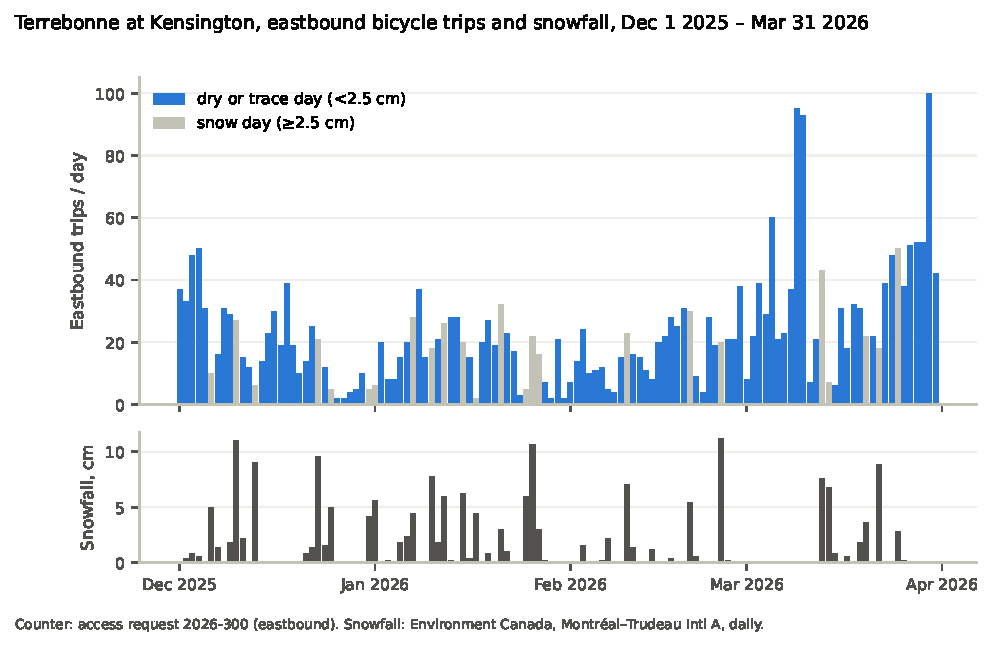
\includegraphics[width=\linewidth]{exposure_winter_2025-26.pdf}
\caption{Daily eastbound trips (top) and snowfall (bottom), December~1,
2025 to March~31, 2026. Grey bars mark days with 2.5~cm or more of snow.}
\end{figure}

\begin{table}[htbp]
\centering\small
\begin{tabular}{lrrr}
\toprule
Season whose CDN loading calendar is applied & Loading days & Eastbound trips & Share \\
\midrule
2015--16 & 21 & 481 & 17\% \\
2016--17 & 30 & 550 & 20\% \\
2017--18 (heaviest in the record, 18.0~M~m$^3$) & 42 & 639 & 23\% \\
2018--19 & 40 & 673 & 24\% \\
2019--20 & 24 & 443 & 16\% \\
2020--21 & 21 & 399 & 14\% \\
2021--22 & 27 & 527 & 19\% \\
2022--23 & 27 & 517 & 19\% \\
2023--24 (lightest, 6.5~M~m$^3$) & 12 & 247 & 9\% \\
2024--25 & 27 & 503 & 18\% \\
2025--26 (7.3~M~m$^3$) & 24 & 410 & 15\% \\
\bottomrule
\end{tabular}
\caption{The 2025--26 daily counts under each season's borough loading
calendar ($\geq$100 loads a day, aligned by calendar date). Only the storm
calendar changes between rows.}
\end{table}

\textbf{The storm days are a minority of the trips.} On the borough's
measured loading days a storm-only closure would have put 410 eastbound
trips into mixed traffic, 15\% of the 2{,}783 an all-winter conversion
affects; on the sector's, 548 (20\%); extended back to the triggering
snowfall, 592 (21\%); on every day with any loading activity at all,
1{,}129 (41\%). Under the most generous snow-day rule in the table, 44\%.
Every definition leaves more than half of the all-winter exposure as trips
on days when no storm closure would have applied.

\textbf{Most winter cycling happens on dry days.} Of the 2{,}783 eastbound
trips, 1{,}699 (61\%) were on the 67 days with no snowfall at all, and
2{,}321 (83\%) on the 97 days with less than 2.5~cm. On the
December--February window, 775 of 1{,}626 (48\%) were on zero-snow days.

\textbf{Cyclists ride on snow days and through loading operations.} Over
the season, mean eastbound trips were 25.4 on dry days, 20.7 on trace days
and 19.2 on days of 2.5~cm or more, and 17.1 on the borough's loading days
against 24.5 on other days. Most of that gap is March: on the
December--February window the figures are 17.2 on dry days, 16.9 on
$\geq$2.5~cm days, and 17.3 on loading days against 18.3 on other days.
Day-to-day, trips correlate with mean temperature ($+0.54$ over the
season) and with snow on the ground ($-0.44$) more than with the day's
snowfall ($-0.12$): cold and accumulated snow suppress cycling more than
the day's fall does. The exceptions are the heaviest storms: the
January~27--31 operation, which followed 16.6~cm in three days, saw 2, 7
and 2 trips on three of its five days.

\textbf{The winter does not change the answer.} Winter 2025--26 was light,
185~cm at Trudeau against a long-run mean near 210, with no day above
11.2~cm and 7.3~million~m$^3$ hauled city-wide, the second-lowest of
eleven seasons (median 12.0; 2017--18, 18.0). The second table applies the
other ten seasons' loading calendars to the same daily counts: the share
ranges from 9\% to 24\%, median 18\%, and the heaviest season on record
gives 23\%. At sector level the eleven seasons give 8\% to 23\%.

\section{In short}

\textbf{On the dry days, the conversion costs cyclists and relieves no
snow constraint.} Sixty-one percent of last winter's eastbound trips
(1{,}699; 48\% on the December--February window) were ridden on days with
no snowfall, when the street's parking supply is not reduced by snowbanks
and no loading operation is under way. Under an all-winter conversion each
of those trips is made in the single remaining traffic lane, between
parked cars on both sides, with the hazards that configuration carries:
less room to pass, and the opening of car doors along the whole block.
Under a storm-only closure none of them is affected. What the conversion
provides on those days is parking on a day when parking is not short of
space for snow; whether that is worth the exposure is a judgement this
note does not make, but the quantities on each side are now known.

\textbf{On the snow days, cycling continues, and the exposure per trip is
greater.} Within deep winter, loading days carried as many eastbound trips
as other days (17 against 18 a day, December to February). These are the
days of reduced traction and visibility, when the margin between a bicycle
and a passing vehicle matters most. Under either option the lane is
unavailable on these days; the difference between the options is entirely
in the dry days above. A closure confined to the loading days would thus
place the trips in mixed traffic on exactly the days the roadway is worst,
and nowhere else; the all-winter conversion adds the rest of the season to
that.

\textbf{Put as a hypothetical.} If the current proposal had been in force
last winter, and assuming that the new configuration would not have
deterred cyclists from riding on Terrebonne, as was predicted at the
October~6 council meeting, the following impacts could be posited:
\begin{enumerate}[nosep]
  \item on the 67 snow-less days, a total of 1{,}699 bike trips would have
    been shifted from a protected bike lane to a driving lane, possibly
    narrower than today's, with parked cars on both sides;
  \item on the remaining 54 days, 1{,}084 bike trips made on days with
    snowfall would have been shifted to the shared driving lane.
\end{enumerate}
The measure is confined to winter, yet over half of last winter's days, 67
of 121, had no snowfall. A dry day can still follow a storm with the
snowbanks not yet cleared; counting every day from a triggering snowfall of
2.5~cm or more to the end of the loading operation that followed in
Terrebonne's own clearing sector, CDN-301, as a day on which snow
constrained parking gives 44 such days and 770 trips, and leaves 77 days
(64\%) and 2{,}013 trips (72\%) on which the lane would have been parking
with no snow on the street to justify it. The same rule on the borough's
loading days, which end a day or two sooner, gives 36 days inside and 85
days (70\%) and 2{,}191 trips (79\%) outside (Table~\ref{tab:season}).
The assumptions are those of the note: the trips are eastbound passages at
Kensington, the direction the councillor said would be converted, and a
floor on use of the street; snowfall is the day's total at Trudeau
airport, and the snow-less days include days with snow on the ground; the
driving lane's width under the winter layout is not in the released file.

\section{Limits}

\textbf{The counter from March~1, 2026.} The counter's eastbound and
westbound totals are balanced to within a few percent in every month from
July~2025 to February~2026 and diverge from March (70\% eastbound in
March, 59--61\% in April and May). The citizen Telraam camera on Terrebonne
at King-Edward, which observes the same roadway, agrees with the loop's
eastbound channel through March but records westbound days of 80 to 190
bicycles where the loop records 10 to 40, after four months in which the
loop counted 1.6 to 2 westbound bicycles for each one the camera saw. The
loop's westbound detection therefore degraded around March~1, and its
counts from that date are lower bounds. The March eastbound figures are
consistent with the camera but are not vouched for separately, which is
why the table also gives the December--February window. Asked on
October~13, 2026 whether the counter was serviced, moved or re-tuned, the
borough's engineering division replied on October~15 that nothing was done
to the loop between mid-February and mid-March 2026, that the only recorded
intervention is a battery replacement in early June with a brief
interruption whose data were reconstituted by the manufacturer, that it
sees no evidence of a technical fault, and that a snow or ice bank on the
westbound side, the side next to the parked cars, may have altered where
people rode. The weekly record places the break in the week of March~2 and
shows the imbalance persisting at 58--61\% eastbound through April and
early May, after the snow was gone, while the camera's directional split
over the same months barely changes; the westbound counts from March~1
therefore remain lower bounds here.

\textbf{The supplier's revisions of the series.} Asked through the
division, the counter's supplier replied on October~21, 2026 (relayed by
the division the same day) that it has revised the site's series five
times since July 2025: redistributions between the two directions for
November~21--26, 2025 and March~9--10, 2026, each keeping the daily total
and replacing the split by the site's historical weekday ratio; an hourly
reconstruction of December~25, 2025; and reconstructions of the missing
bicycle data of May~29--31, 2026 and of the missing motor-vehicle data of
June~8--9, 2026, estimated from correlated counters elsewhere in the city.
The hourly record used here (export of June~4, 2026) contains the November
redistribution but not the March one: March~9 and 10 stand at 82\% and 80\%
eastbound, like the days around them. Redistributing those two days, which
had no snowfall and no loading, moves about 67 passages from eastbound to
westbound; the eastbound total becomes about 2,716 and the share outside
constraint days 71.6\%, unchanged at the rounding. No other figure in this
note is affected. The supplier also reports no abnormal gap between the
directions on its side apart from the November days, and four bicycle
channels on the site where the export has two; the mapping of the export's
columns to those channels has been asked of the division. The releases,
the check and the effect on each figure are set out in the note of
October~21, 2026 in the 2026-581 folder of the same repository
(\texttt{derived/counter\_revisions\_and\_westbound\_channel\_2026-10-21.md}).


\textbf{One winter, one station, one counter.} The counter stands at one
point on a 2.45~km lane; use varies along it. Trudeau airport is 12~km
west of Terrebonne; day-level snowfall is well correlated across the
island, but amounts on NDG streets can differ. The loading days are the
borough's and sector CDN-301's; the lane's last blocks, Draper to
Girouard, lie in sector CDN-111 and are outside the sector figures, and
sector boundaries may have changed
between contracts (only the 2025--26 polygons were checked; CDN-301
appears as 301A and 301B in 2019--20 and is combined). The multi-season
table holds the cyclists fixed and changes only the calendar; in a heavier
winter fewer people would have ridden on the storm days themselves, which
makes those rows conservative in the other direction.

\textbf{What this note does not measure.} The parking side: how many
spaces are lost to snowbanks on which days, and how many vehicles need
them. The City's record contains no such count. This note measures what
the cyclists' side of an all-winter and a storm-only closure would have
been; the comparison of benefits is for the reader.

\section{Files}

All inputs and the script that produces every number above are in
\doc{2026-300/derived/}{2026-300/derived/}: the counter record summed to
days by direction; the merged daily table with weather and loading
activity; the City's loading record summed by season, day, borough and
sector; the two ECCC annual files; the sector lookup; and
\texttt{exposure\_analysis.py}, which regenerates the tables and the figure
from those files. The counter's hourly workbook and the borough's response
letter are in \doc{2026-300/raw/}{2026-300/raw/}, exactly as received.

\end{document}
